\begin{tikzpicture}
	\onslide<1->{\node at (1.0,0.0) (figa)  { 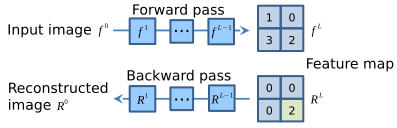
\includegraphics[scale=0.4]{images/3_2_1.jpg}};}
	\onslide<2->{\node at (0,-2) (figb)  { \includegraphics[scale=0.5,trim={0cm 9cm 0cm 0cm},clip=true]{images/3_2_2.pdf}};}
	\onslide<3->{\node at (0,-4) (figc)  { \includegraphics[scale=0.5,trim={0cm 6cm 0cm 3cm},clip=true]{images/3_2_2.pdf}};}
	\onslide<4->{\node at (0,-6) (figd)  { \includegraphics[scale=0.5,trim={0cm 0cm 0cm 9cm},clip=true]{images/3_2_2.pdf}};}
\end{tikzpicture}